\section{Design}
\label{sec:design}
We describe the evolution of the design of \system{} starting with an initial strawman approach.  We then 
alter the design as we address each of the design goals discussed in the previous section (and in Table \ref{tab:design_goals}), which brings us 
to a complete design.

\subsection{Strawman: Hiding Information From CDN}
\label{sec:obfuscate_content}
To prevent an inside attacker or overreaching government from learning information, the CDN 
must not have the knowledge of what content it is caching.  Therefore, the content {\it and} the 
associated URL must be obfuscated before they enter the CDN.  

\paragraph{Encrypt Content}  The content can be obfuscated by encrypting it with a key that is not 
known to the CDN.  Because this must be done prior to any caching, the content publisher 
has to generate some key $k$ to encrypt the content with.  Then this encrypted (and subsequently 
obfuscated) content is then sent to the CDN\footnote{Most CDNs
allow the publisher to decide on a push or pull model, but this makes no difference in our 
system design.} and stored in its caches.  
Additionally, if the domain supports HTTPS requests, then the content publisher must also encrypt the 
associated certificate with the same key $k$.  This content and certificate must be decrypted after 
it leaves the CDN; the client could decrypt the certificate and check its validity.  If valid, then 
the client uses $k$ to decrypt the content.  

\paragraph{Obfuscate URL} Encrypting the content alone does not hide much from the CDN; the content 
identifier, or URL, must also be obfuscated, otherwise the CDN can still reveal information about 
which clients accessed which URLs (which is indicative of the content).  In obfuscating the 
URL, the result should be a fixed, and relatively small size; these requirements are to preserve 
storage space and to prevent the adversary from guessing the URL based on the length of the obfuscated 
URL.  Hashing the URL provides these 
properties, and hides the actual URL from the CDN. With obfuscated content and 
URLs, the CDN does not know what content a given client is accessing.

\paragraph{Client Anonymization}  The CDN may not know the content that a client is accessing, but it 
still knows information about the clients that are accessing any content at the CDN.  It knows 
where the clients are located and how many times they are accessing any content.  To address this, 
a client can simply use an anonymizing proxy or VPN when accessing content.  This hides a certain 
amount of information about the client, including the client's location and a direct link of 
client to content request.

This strawman approach obfuscates content from the viewpoint of the CDN, which also allows the CDN 
to claim plausible deniability when served with a subpoena.  Despite only caching encrypted and obfuscated 
content and identifiers, the CDN still has knowledge of which clients are requesting any content and how often 
they are requesting content.  Unfortunately, this approach raises 
many questions: are anonymizing proxies/VPNs trustworthy?, should clients be trusted to know $k$?, 
can any jurisdiction still subpoena the CDN for information (presumably the CDN has locations in many 
countries and clients in many countries)?, and if a subpoena is served, what is learned?

\begin{figure}[t!]
\centering
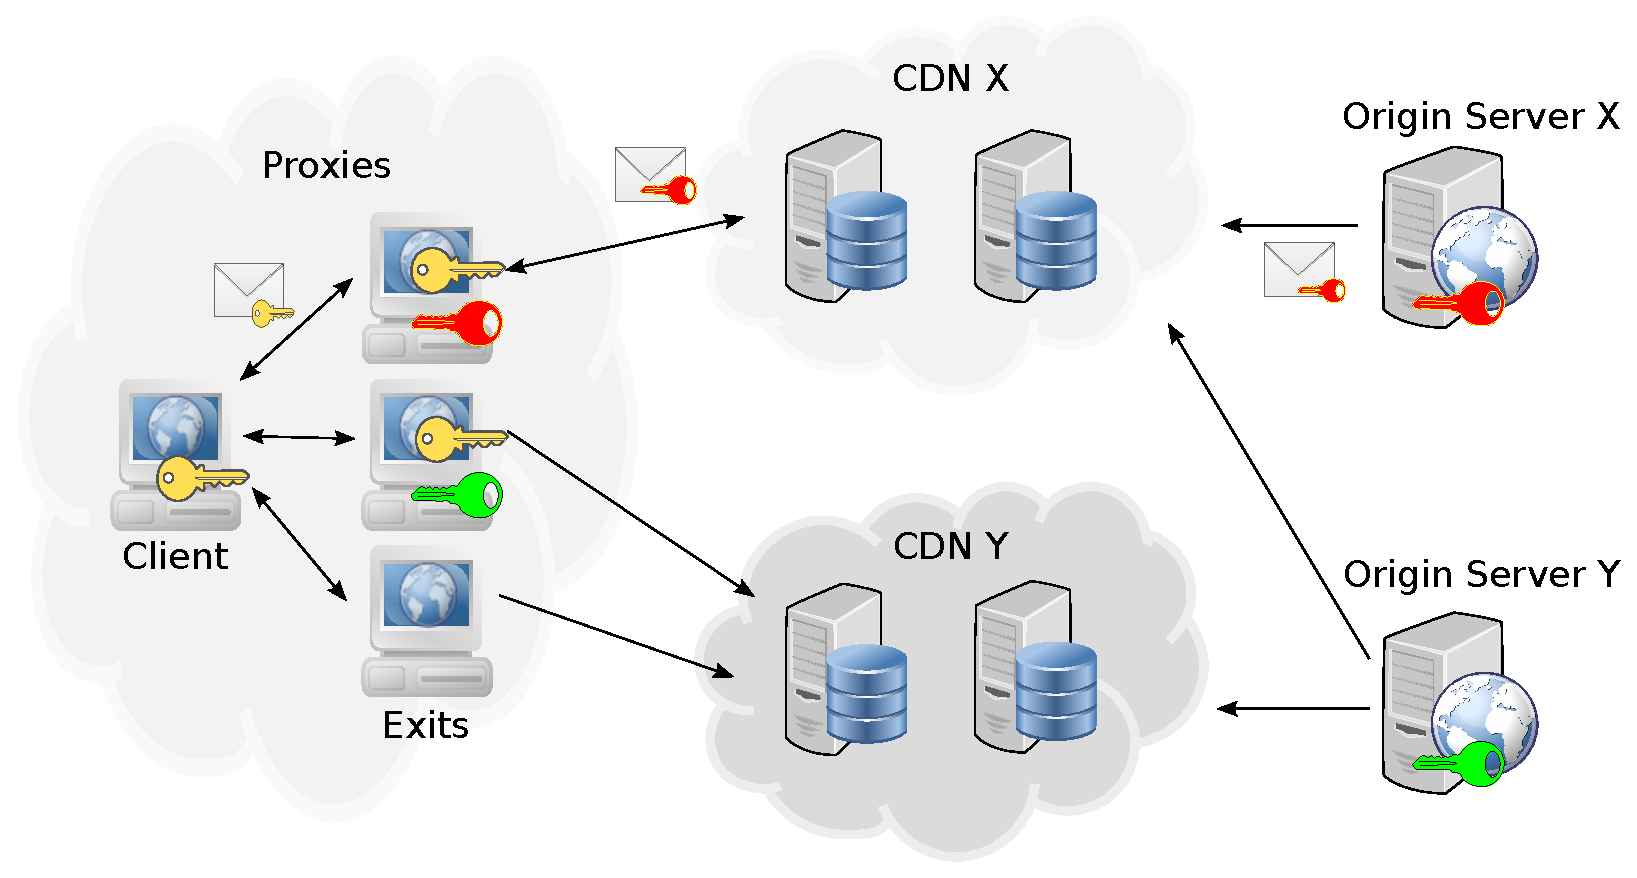
\includegraphics[width=.5\textwidth]{ocdn_overview_new2}
\caption{The relationships between clients, the CDN, proxies, and content publishers in 
\system{}.}
\label{fig:ocd_overview}
\end{figure}

\subsection{System of Proxies}
\label{sec:proxies}

While a VPN or anonymizing proxy may hide a client's identity from the CDN, it puts a large amount of trust in the VPN provider (or proxy), which 
has knowledge of each client's IP address, and what content each client is requesting.  This can be addressed 
by using a system of proxies instead of a VPN provider; by introducing a set of proxies that requests are 
forwarded through before reaching the CDN, clients no longer have to trust a single entity (VPN provider), and 
can achieve a level of anonymity.

\paragraph{Hiding Clients' Identities} By replacing the use of an anonymizing proxy or VPN with the use of 
a series of proxies---some of which are supplied by \system{} and some of which are simply other clients---, 
the system can provide unlinkability of client to her requests/responses. There are two distinct sets of 
proxies: 1) exit proxies and 2) client proxies.  We discuss in Section \ref{sec:xx} how these can be run by different 
entities.  Exit proxies provide a way of requesting encrypted content from CDNs; these proxies store the keys generated 
by content publishers (as described in the strawman approach).  Client proxies provide 
a way for any client to route her traffic to an exit proxy, while hiding her identity.  When requesting content, she 
generates a route that can include a series of client proxies and must include an exit proxy, and each client proxy 
forwards the request based on this route.  In order for other clients to be unsure of the original requestor client's 
identity, the original requestor client can lie about the route; she can lie by including other client proxies 
in the route before herself.  For example, if she has identity {\it C}, she could generate a route to exit proxy {\it E} that 
looks like 

\[C \rightarrow G \rightarrow F \rightarrow E\] 

\noindent She can hide her identity from {\it G} and {\it F} by using the route 

\[D \rightarrow A \rightarrow C \rightarrow G \rightarrow F \rightarrow E\]  

\noindent Neither {\it G}, {\it F}, or {\it E} know who the original requestor was; from {\it E}'s point of 
view, the original requestor could have been {\it D}, {\it A}, {\it C}, {\it G}, or {\it F}.  By using a series of 
client proxies, or even just that a client {\it can} use a series of client proxies, the identity of the client is 
hidden from other clients, exit proxies, and the CDN.  Using both types of proxies is essential for a couple of 
reasons: 1) just using client proxies would disallow any client behind a NAT, or any mobile client from joining 
the system and 2) just using exit proxies would put too much trust in the proxies, as they would know the identity 
of each client, and what content each client is requesting.

%As it is still unclear which jurisdiction is legally allowed to subpoena information from the CDN (such as which 
%clients are accessing any content distributed by the CDN), this 
%system should complement the legal framework; it should make clear which jurisdictions are allowed 
%which information, and also prevent an overreaching government from demanding data.  This 
%can be addressed by introducing a closed system of proxies, where a client uses a single proxy when requesting 
%content---not only does this proxy provide a level of client anonymity, but also decides which jurisdiction 
%the data falls under.  

%\paragraph{Proxy in Client's Jurisdiction} By replacing the use of an anonymizing proxy or VPN with the use 
%of a proxy---one that is part of \system{} and supplied to clients based on their location---, the system can specify which juridiction each client falls under.  For example, 
%each country could have a set of proxies, where all clients in each country use one of the proxies that 
%is located in their country.  This should allow the client's jurisdiction to serve a subpoena for information 
%passing through the specific proxy that a client uses in the client's jurisdiction in 
%necessary criminal investigations, but prevents any other jurisdiction from demanding data on the same 
%client because the subpoena must be served for a specific proxy.  While it appears that the source of 
%trust is simply shifted from the CDN to the proxy, the use of this proxy is essential in 
%the system design for a number of reasons.  First, the use of proxies distributes trust; instead of a 
%central entity, the CDN, having access to all information, it is now a set of proxies that each have 
%access to some subset of information.  Each proxy only knows information about a much smaller set of clients.  
%Additionally, the proxy does not cache content or keep state, whereas the CDN does both of these.  Apart 
%from addressing jurisdictional issues, proxies also improve usability; instead of each client having knowledge 
%of each $k$ for each domain, each proxy could have knowledge of each $k$.  This means that clients would 
%not have to keep track of secret knowledge, and overall, the number of entities that know this secret key 
%is much smaller (as the number of proxies is significantly smaller than the number of clients).  Lastly, 
%the proxy can perform attack detection and prevention before the attack even reaches the CDN; more optimizations 
%made possible by the use of proxies are discussed in Section \ref{sec:optimizations}.

\paragraph{Decouple Content Distribution from Decision of Trust} Using proxies also separates the issues of 
trust and content distribution.  A client no longer needs to trust the CDN, which all other clients would 
need to trust as well.  Now the client can simply trust the set of proxies to perform the correct actions, but 
does not need to trust anyone to keep her information private.  All proxies in the system are completely separate entities 
from the CDN (and sometimes even from each other proxy).  Therefore this design allows a client to decouple these 
issues, but still access cached content at the CDN.

\paragraph{Usability} Instead of each client having knowledge 
of each $k$ for each domain, each proxy could have knowledge of each $k$.  This means that clients would 
not have to keep track of secret knowledge, and overall, the number of entities that know this secret key 
is much smaller (as the number of proxies is significantly smaller than the number of clients).  Lastly, 
the proxy can perform attack detection and prevention before the attack even reaches the CDN; more optimizations 
made possible by the use of proxies are discussed in Section \ref{sec:optimizations}.

\subsection{Key Use and Management}
\label{sec:keys}
The design has evolved into a system where: 1) the CDN does not know the content, the content identifier, 
or which clients are accessing any content, 2) the client's data is only subject to subpoenas in her jurisdiction 
(or the jurisdiction of the proxy), 3) trust has been distributed, as opposed to centralized.  There are still 
some remaining security vulnerabilities that must be addressed.  First, simply hashing the URL allows an attacker who simply 
wishes to guess whether the obfuscated URL is a specified plaintext URL or not.  Second, the shared key $k$ for each content 
publisher has the potential to be compromised, and therefore, OCDN must have a way to create new keys and replace 
old keys with the new ones.

\paragraph{Adding Secrecy to URL Obfuscation} According to the strawman approach, the URL is obfuscated via hashing.  Unfortunately, 
an attacker could guess what the content identifier is by hashing his guesses and comparing with the hashes stored in the 
CDNs caches.  To mitigate this vulnerability, the content publisher should incorporate the use of the shared key $k$ in the 
hash of the URL by using a hash-based message authentication code (HMAC).  This provides the property of fixed length 
identifiers, which does not reveal information about the plaintext identifiers, while obfuscating and preventing 
against guessing attacks.  

\paragraph{Minimizing Shared Key Holders} If a single shared key $k$ associated with a single content publisher gets 
compromised, then all proxies have a compromised $k$ for that content publisher.  A naive approach to address this 
is for the content publisher to generate a different $k$ for each proxy; unfortunately, this defeats the purpose of 
CDNs caching content.  The approach \system{} takes is for each content publisher to generate a single shared key $k$, 
and for a single proxy to hold that key; this maximizes the use of the CDNs caches.  The shared key is assigned 
to an exit proxy based on consistent hashing~\cite{????}, which provides load balancing properties.  For more popular 
content, it may be useful to have more than one exit proxy serving that content; in this case, a few exit proxies can 
hold this key.  We discuss this case in more detail in Section \ref{sec:xx}.

\paragraph{Key Churn} To protect against attacks when a content publisher's shared key $k$ is compromised, the publisher
should generate a new key $k$ and encrypt her content under the new key.  Keys have an expiration timestamp that indicates 
when a key is no longer valid; the publisher should generate a new key when a current key has expired.  Additionally, 
proxies should obtain the new key when a current key expires.  

%\paragraph{Increasing the Number of Keys} If a single shared key $k$ associated with a single content publisher gets 
%compromised, then all proxies have a compromised $k$ for that content publisher.  By increasing the number of shared 
%keys that a content publisher uses to encrypt her content, this decreases the fraction of proxies that use a 
%compromised key given that one of the keys is compromised.  Instead of a content publisher encrypting content with a 
%single key, she will encrypt a copy of the content with different keys.  If there are $n$ shared keys, then there 
%will be $n$ copies of the content, where each copy is encrypted with a different shared key.  To maximize security, each proxy should share a
%different $k$ with the content publisher; unfortunately, this defeats the purpose of CDNs caching content.  If each 
%proxy is requesting a unique copy of the content, then cache hit rates decrease and performance becomes worse.  To make 
%a tradeoff between security and performance, there should be $n$ keys where $1 < n < |proxies|$, such that subsets of 
%proxies share the same shared key $k$ with the content publisher.  If one of these shared keys is leaked (or otherwise learned), only that 
%subset of proxies that use that shared key must get a new key.  \\

The resulting system is the basis of \system{}, and the high-level view of the system is shown in Figure \ref{fig:ocd_overview}, 
which can be compared to what CDNs look like today (Figure \ref{fig:basic_cdn}).  The next section describes \system{} in more 
detail and outlines the specific steps for publishing and retrieving content.
